\documentclass[a4paper,14pt]{extarticle}


\usepackage[utf8]{inputenc}
\usepackage[T2A]{fontenc}
\usepackage[english,russian]{babel}
\usepackage{ragged2e}
\usepackage[utf8]{inputenc}
\usepackage{hyperref}
\usepackage{minted}
\setmintedinline{frame=lines, framesep=2mm, baselinestretch=1.5, bgcolor=LightGray, breaklines,fontsize=\scriptsize}
\setminted{frame=lines, framesep=2mm, baselinestretch=1.5, bgcolor=LightGray, breaklines,fontsize=\scriptsize}
\usepackage{xcolor}
\definecolor{LightGray}{gray}{0.9}
\usepackage{graphicx}
\usepackage[export]{adjustbox}
\usepackage[left=1cm,right=1cm, top=1cm,bottom=1cm,bindingoffset=0cm]{geometry}
\usepackage{fontspec}
\usepackage{ upgreek }
\usepackage[shortlabels]{enumitem}
\usepackage{adjustbox}
\usepackage{multirow}
\usepackage{amsmath}
\usepackage{amssymb}
\usepackage{pifont}
\usepackage{pgfplots}
\usepackage{longtable}
\usepackage{array}
\graphicspath{ {./images/} }
\makeatletter
\AddEnumerateCounter{\asbuk}{\russian@alph}{щ}
\makeatother
\setmonofont{Consolas}
\setmainfont{Times New Roman}

\newcommand\textbox[1]{
	\parbox{.45\textwidth}{#1}
} 

\newcommand{\specialcell}[2][c]{%
	\begin{tabular}[#1]{@{}c@{}}#2\end{tabular}}

\begin{document}
\pagenumbering{gobble}
\begin{center}
    \small{
        \textbf{МИНИCТЕРCТВО НАУКИ И ВЫCШЕГО ОБРАЗОВАНИЯ РОCCИЙCКОЙ ФЕДЕРАЦИИ}\\
        ФЕДЕРАЛЬНОЕ ГОCУДАРCТВЕННОЕ БЮДЖЕТНОЕ ОБРАЗОВАТЕЛЬНОЕ УЧРЕЖДЕНИЕ\\ВЫCШЕГО ОБРАЗОВАНИЯ \\
        \textbf{«БЕЛГОРОДCКИЙ ГОCУДАРCТВЕННЫЙ ТЕХНОЛОГИЧЕCКИЙ\\УНИВЕРCИТЕТ им. В. Г. ШУХОВА»\\ (БГТУ им. В.Г. Шухова)} \\
        \bigbreak
        
\includegraphics[width=70mm]{log}\\
        ИНСТИТУТ ИНФОРМАЦИОННЫХ ТЕХНОЛОГИЙ И УПРАВЛЯЮЩИХ СИСТЕМ\\}
\end{center}

\vfill
\begin{center}
    \large{
        \textbf{
            Лабораторная работа №3}}\\
    \normalsize{
        по дисциплине: Основы ИИ \\
        тема: «Муравьиный алгоритм»}
\end{center}
\vfill
\hfill\textbox{
    Выполнил: ст. группы ПВ-223\\Пахомов Владислав Андреевич
    \bigbreak
    Проверили: \\пр. Твердохлеб Виталий Викторович
}
\vfill\begin{center}
    Белгород 2025 г.
\end{center}
\newpage
\underline{\textbf{Цель работы: }}изучение и исследование параметров муравьиного
алгоритма на примере решения задачи коммивояжера.\\
\begin{center}
\textbf{Ход выполнения работы}
\end{center}


\includegraphics[width=140mm]{algorythm}\\

\href{https://github.com/IAmProgrammist/ai_basics/tree/lab3}{Ссылка на репозиторий}\\

Опыт №1: обычный сценарий\\
$N = 3$\\
$a = 1$\\
$b = 3,5$\\
$\rho = 0,2$\\

\includegraphics[width=140mm]{report1}\\
Обычный сценарий. Алгоритм не всегда находит оптимальный маршрут, особенно если в нём много альтернативных путей.
Но в целом оптимально.\bigbreak

Опыт №2: кадровые перестановки\\
$N = 1/20$\\
$a = 1$\\
$b = 3,5$\\
$\rho = 0,2$\\
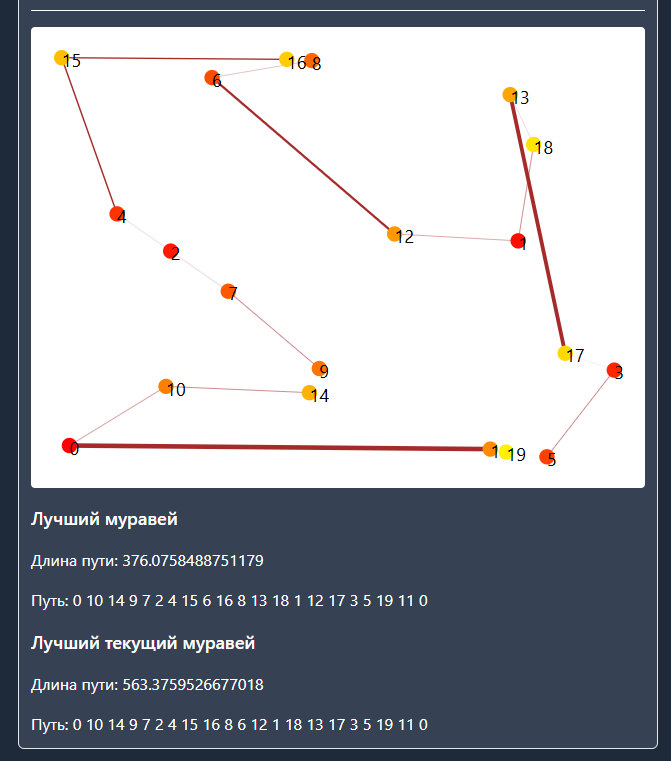
\includegraphics[width=140mm]{report21}\\
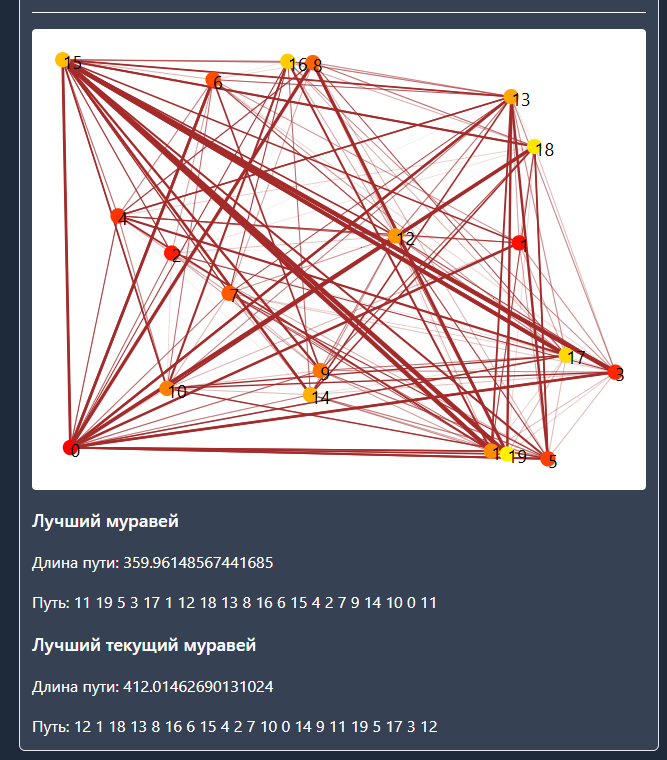
\includegraphics[width=140mm]{report22}\\
Слишком маленькое число муравьёв даёт слишком маленькое количество вариантов. В итоге мы получаем результат, очень далёкий от 
оптимального, а альтернатив очень мало. Зато это очень быстро. При большом количестве муравьёв у программы слишком много вариантов, и алгоритм мало
чем отличается от полного перебора всех путей. К тому же, система начинает очень сильно "тормозить". Оптимальное значение ~5.\bigbreak

Опыт №3: доверься коллегам\\
$N = 3$\\
$a = 0,01/100$\\
$b = 3,5$\\
$\rho = 0,2$\\
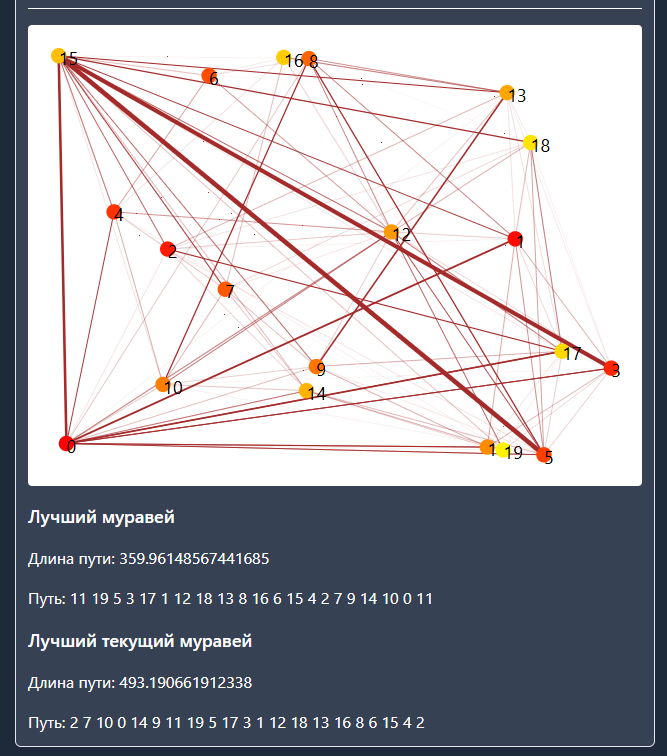
\includegraphics[width=140mm]{report31}\\
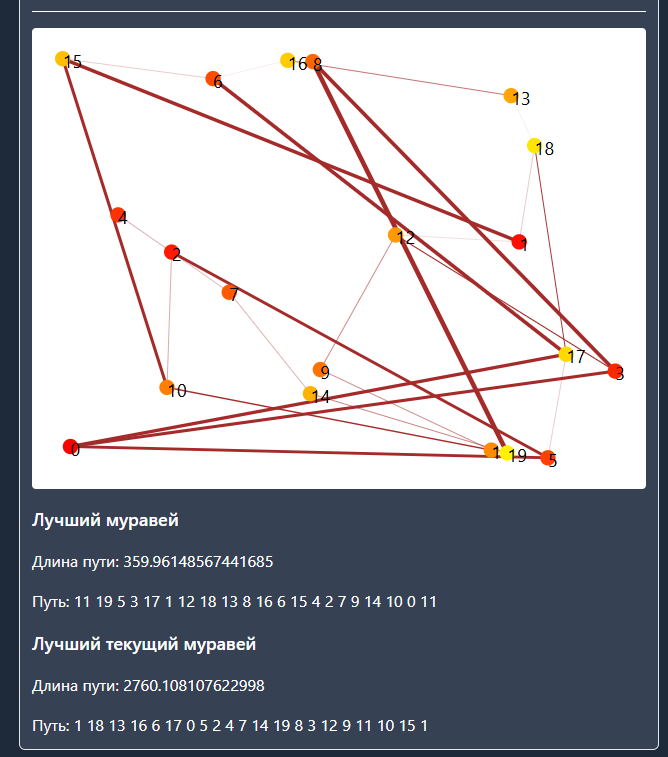
\includegraphics[width=140mm]{report32}\\
При маленьком $a$ алгоритм находит оптимальные рёбра, однако очень с большим количеством ребёр он не может "определиться", итоговое решение шумное и 
не предоставляет переиспользуемую сеть, между элементами очень много связей. При большом же $a$ алгоритм не получает альтернативных мнений
относительно путей, и придерживается уже положенных путей. Конечно, такой вариант будет крайне неоптимальным.\bigbreak

Опыт №4: доверяй но проверяй\\
$N = 3$\\
$a = 1$\\
$b = 0,01/100$\\
$\rho = 0,2$\\
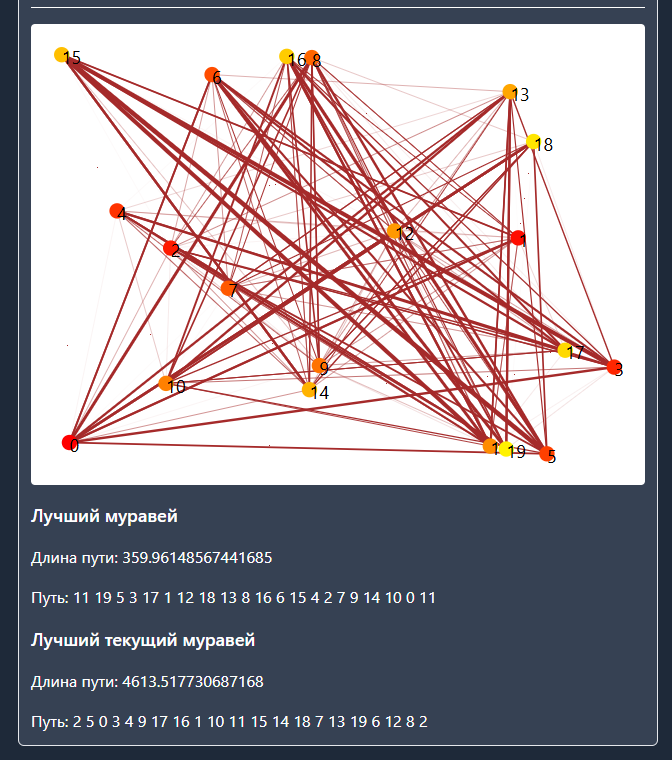
\includegraphics[width=140mm]{report41}\\
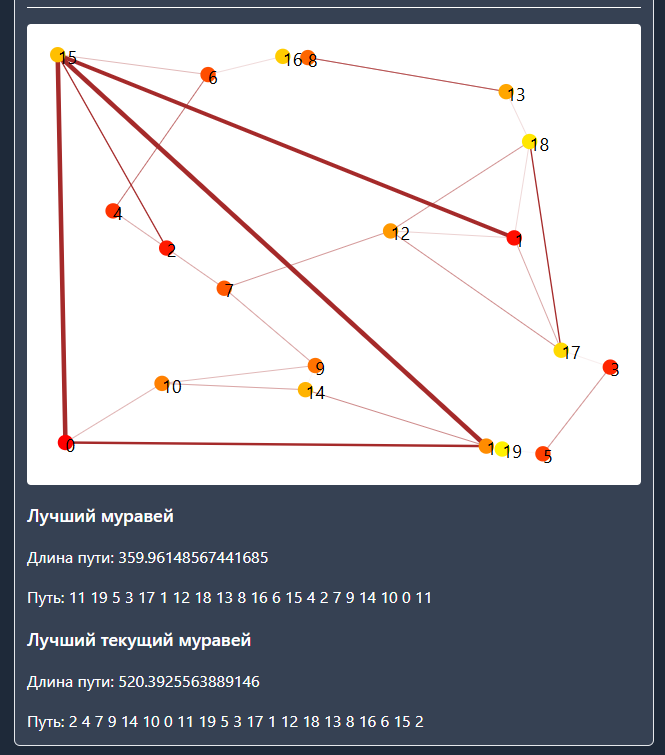
\includegraphics[width=140mm]{report42}\\
При очень маленьком $b$ у муравья совсем нет собственной воли и логики, он ходит только по "вонючим" местам, конечно же такой вариант
будет неоптимальным и будет содержать очень длинный путь. При большом $b$, казалось бы, кажется что муравей должен найти путь 
очень быстро, он всегда предпочитает наиболее близкий пункт. И действительно, решение оказывается лучше, чем при маленьком 
$b$. Но порой следовать только самому короткому пути - не лучшее решение. Иногда стоит больше доверять пройденному опыту.\bigbreak


\textbf{Вывод: } в ходе лабораторной работы изучили и исследовали параметры муравьиного
алгоритма на примере решения задачи коммивояжера.

\begin{minted}{Rust}
use std::{error::Error, f64::INFINITY, future, sync::{mpsc::channel, Arc, RwLock, RwLockReadGuard}, vec};

use rand::Rng;
use threadpool::ThreadPool;

use crate::utils::{ACOConfig, ACOPaths, Ant};

pub async fn aco(config: &ACOConfig, paths: & mut Arc<dyn ACOPaths>) -> Result<Ant, Box<dyn Error>> {
    let mut handles = Vec::new();
    {
        let field = Arc::new(RwLock::new(paths.clone()));
        
        let cpu_count = num_cpus::get_physical();
        let pool = ThreadPool::new(cpu_count);
        let ants_amount = config.ants;
        
        for _worker in 0..ants_amount {
            let (tx, rx) = oneshot::channel();
            let field_clone = Arc::clone(&field);
            let config = config.clone();

            let handle = tokio::task::spawn_blocking(move || {
                let mut rng = rand::rng();
                let field_read = field_clone.read();
                let mut ant = Ant::new();
                if field_read.is_err() {
                    let _ = tx.send(ant);
                    return;
                }

                // Если инициализация, ставим в случайную точку. Иначе - в ноль.
                let field_read = field_read.unwrap();
                //if field_read.is_fresh() {
                    ant.visited.push(rng.random_range(0..config.ants));
                //} else {
                //    ant.visited.push(config.begin_city.unwrap_or(0));
                //}
                loop {
                    let field_read = field_clone.read().unwrap();
                    match find_next_city(&config, &field_read, &ant) {
                        Ok(city_index) => {
                            ant.len += field_read.get_distance(ant.visited[ant.visited.len() - 1], city_index).unwrap_or(0.0);
                            ant.visited.push(city_index);
                            if ant.visited.len() == field_read.len() {
                                ant.visited.push(ant.visited[0]);
                                let _ = tx.send(ant);
                                return;
                            }
                        },
                        Err(e) => {
                            println!("Whoopsie for ant: {}", e);
                            let _ = tx.send(Ant::new());
                            return;
                        }
                    }
                }
            });

            handles.push((rx, handle));
        }

        pool.join();
    }
    let mut best_ant = Ant::new();
    best_ant.len = INFINITY;
    {
        for (rx, handle) in handles {
            // Waiting for spawn to be completed
            let _ = handle.await;

            let ant = rx.await.unwrap_or(Ant::new());
            if ant.visited.len() == 0 {
                continue;
            }

            if ant.len < best_ant.len {
                best_ant = ant.clone();
            }
            
            let paths = Arc::get_mut(paths).ok_or("Failed")?;

            let feromone_added = get_ant_path_feromone(config, paths, &ant);

            for path_index in 0..(ant.visited.len() - 1) {
                paths.set_feromone_intensity(feromone_added + paths.get_distance(ant.visited[path_index], ant.visited[path_index + 1]).unwrap_or(0.) * config.evaporation_coefficient, 
                ant.visited[path_index], 
                ant.visited[path_index + 1])?;
            }
        }

        let paths = Arc::get_mut(paths).ok_or("Failed")?;
        evaporate(config, paths)?;
    }

    Ok(best_ant)
}

fn find_next_city(config: &ACOConfig, paths: &RwLockReadGuard<'_, Arc<dyn ACOPaths>>, ant: &Ant) -> Result<usize, Box<dyn Error>> {
    let mut probs = vec![0.; 0];
    let mut indices = vec![0; 0];
    let mut denom: f64 = 0.;
    let ant_current_index = ant.visited.last().ok_or("Ant should have at least one point")?;
    let mut rng = rand::rng();

    for city_index in 0..paths.len() {
        if let Some(_) = ant.visited.iter().find(|visited_city_index| **visited_city_index == city_index) {
            continue;
        }

        indices.push(city_index);
        let product = 
            paths.get_feromone_intensity(*ant_current_index, city_index)?.powf(config.feromone_weight) * 
            (1. / paths.get_distance(*ant_current_index, city_index)? as f64)
            .powf(config.heuristic_coefficient);
        denom += product;
        probs.push(product);
    }

    if denom == 0.0 {
        return Err("Luck is not on your side, cowboy".into());
    }

    probs = probs.iter().map(|pr| pr / denom).collect();
    let probability_sum = probs.iter().copied().reduce(|acc, e| acc + e).unwrap_or(0.);
    let curr_prob = rng.random_range(0.0..probability_sum);

    let mut left_prob: f64 = 0.;
    for allowed_city_index in 0..probs.len() {
        if left_prob <= curr_prob && curr_prob <= left_prob + probs[allowed_city_index] {
            return Ok(indices[allowed_city_index])
        }

        left_prob += probs[allowed_city_index];
    }

    Ok(indices[0])
}

fn get_ant_path_feromone(config: &ACOConfig, paths: &mut dyn ACOPaths, ant: &Ant) -> f64 {
    config.q / get_ant_path_length(paths, ant)
}

fn get_ant_path_length(paths: &mut dyn ACOPaths, ant: &Ant) -> f64 {
    let mut path_len = 0.0;
    
    for path_index in 0..(ant.visited.len() - 1) {
        path_len += paths.get_distance(ant.visited[path_index], ant.visited[path_index + 1]).unwrap_or(0.);
    }

    path_len
}

fn evaporate(config: &ACOConfig, paths: &mut dyn ACOPaths) -> Result<(), Box<dyn Error>> {
    for i in 0..paths.len() {
        for j in 0..paths.len() {
            paths.set_feromone_intensity(paths.get_feromone_intensity(i, j)? * (1. - config.evaporation_coefficient), i, j)?;
        }
    }

    Ok(())
}
\end{minted}

\end{document}